\xchapter{Work Proposal}{}\label{cap:3}

\section{The RESCUER Project}

Our research fits in the scope of a larger research project named RESCUER \footnote{\url{http://www.rescuer-project.org/}}, which aims at developing an inter-operable solution that supports command centres in quickly managing emergencies and crisis based on reliable and intelligent analysis of crowdsourcing information mashed up with open data. Two application scenarios are under investigation and support emergency and crisis management in: i) Industrial areas, such as chemical parks; and ii) Large-scale events, such as the Olympic Games.

\begin{figure}[htb]
\begin{center}
  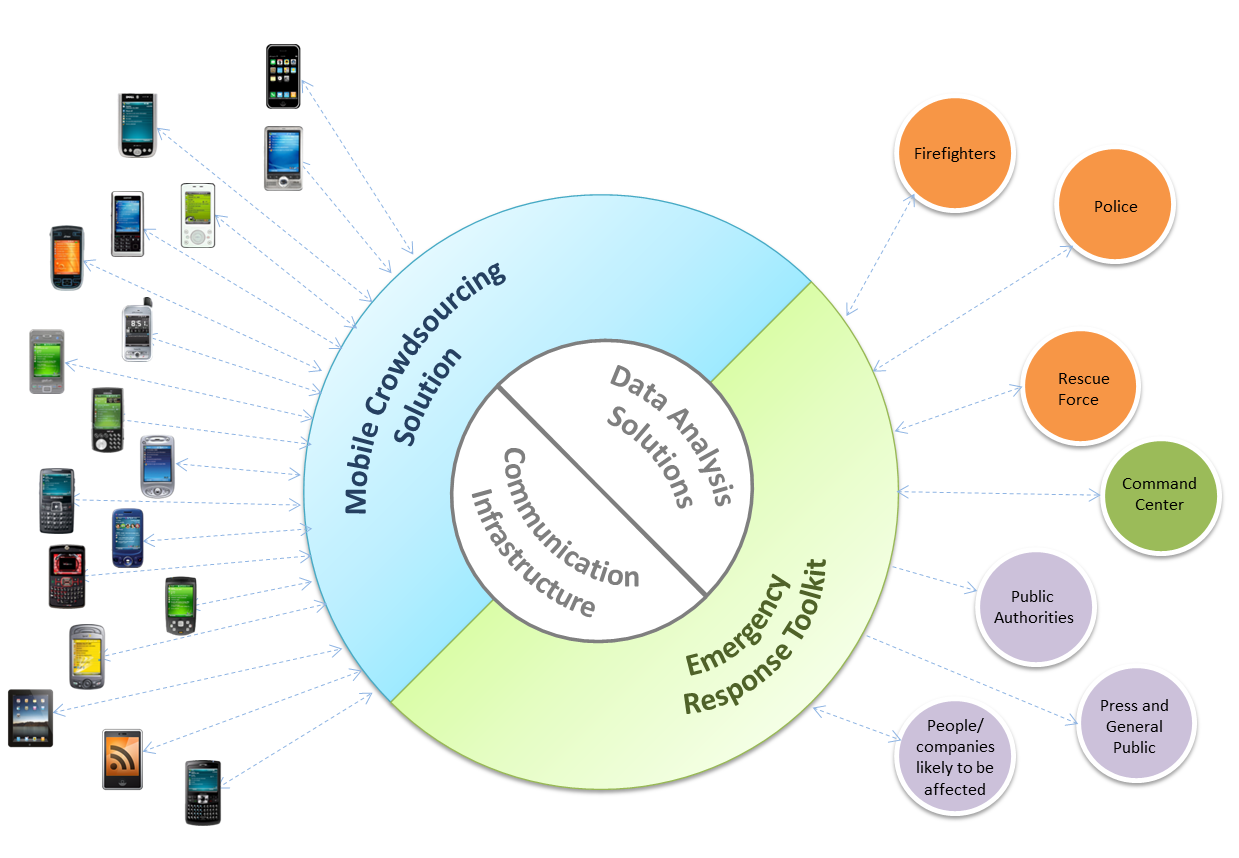
\includegraphics[width=0.7\linewidth, keepaspectratio]{rescuerConcept}
\caption{RESCUER Conceptual Model}
\label{fig:rescuerConcept}
\end{center}
\end{figure}

Figure \ref{fig:rescuerConcept} presents the conceptual view of the Rescuer project. The project was divided into 4 main components: Mobile Crowdsourcing Solution (MCS), Data Analysis Solutions (DAS); Communication Infrastructure and Emergency Response Toolkit (ERTK). 

The MCS is way to receive or send information by the crowd. The users of MCS can be an operational force actuating in mitigating the effects of the crisis or a civilian near of the incident place.

In order to guarantee that the information will be send or received in a suitable time and even when traditional communication infrastructure are overloaded, the Rescuer Project have the Communication Infrastructure module.

The DAS module is responsible to integrating data from the different profiles as well as for combining, filtering, and analysing crowdsourcing information mashed up with open data. 

Finally, the ERTK module provide the command centre with the updated and relevant information, in the appropriate format, to support decision-making in the different phases of an emergency and allow the dissemination of orientations to the affected people and reliable information in the course of emergency.




\section{Collecting Information}

We collected information on how public communication occurs during an emergency from the user organisations involved in RESCUER Project, either as official partners or as collaborators. 

To get this information, a workshop was held with the presence of representatives of Camaçari Industrial Development Committee (COFIC)\footnote{http://coficpolo.com.br/}, FireServ\footnote{http://www.fireserv.at/} and the Command and Control Centre of the Public Safety \& Security Department of the State of Bahia (CICC-BA). COFIC was in charge of providing information from the perspective of industrial parks in Brazil; Fireserv provided information not only from the perspective of industrial parks in Europe, but also from the perspective of large-scale events in this region; and CICC-BA brought the perspective of large-scale events in Brazil.

The workshop was conducted using the Brainstorm technique \cite{diehl1991productivity} and its goal was to answer the
following questions:

\begin{itemize}
   \item What are the stakeholders for the public communication of emergencies?
   \item What is the relevant information in this scenario?
   \item In which emergency phases should the identified information be sent?

 \end{itemize}


Furthermore, we analyse communication templates and processes provided in the partners’ manuals of security. Next, we show the results we achieved.

\subsection*{What are the stakeholders for the public communication of emergencies?}

Inside of Rescuer Project, two activities were conducted, among other things, to identify the the target audience of public communication: the Task D.1.2 Requirements Specification \cite{rescuerD11} and the Task D.4.1 Model of Organisational Behaviour and Structures in Emergencies \cite{rescuerD41}. 

Based on the list of stakeholders presented in this two tasks we elaborated an initial list of stakeholders to receive public communications: Employee / Visitor, Neighbour Community, Press, Public Authority. In addition to informing the aforementioned stakeholders, it is important to keep the public that is not directly involved in the emergency (a.k.a. General Public) informed, as this may reduce anxiety, uncertainty and prepare people for actions they should take in an emergency \cite{cdc2014}.

Workshop participants were requested to refine the initial list of public communication stakeholders, by confirming that the proposed stakeholders were relevant in real-world scenarios; detailing the list, if necessary; and informing stakeholders not covered by the initial proposal.

Workshop participants judged as necessary to replace public authority by politician and environmental department. The last is only applicable to industrial parks. The final list of public communication stakeholders is as follows:


\begin{itemize}
   \item Employee / Visitor;
   \item Neighbour Community;
   \item Press;
   \item Politician;
   \item Environmental Department (exclusive for Industrial Park).
        
 \end{itemize}


\subsection*{What is the relevant information in this scenario?}

\begin{table}[]
\centering
\caption{Stakeholders x Information needs}
\label{stkInformacao}
\begin{tabular}{|c|c|c|c|}
\hline
\rowcolor[HTML]{9BBB59} 
\cellcolor[HTML]{9BBB59}{\color[HTML]{FFFFFF} }                                                                                           & \multicolumn{3}{c|}{\cellcolor[HTML]{9BBB59}{\color[HTML]{FFFFFF} Stakeholder}}                                                                                                                                                                                                                       \\ \cline{2-4} 
\multirow{-2}{*}{\cellcolor[HTML]{9BBB59}{\color[HTML]{FFFFFF} \begin{tabular}[c]{@{}c@{}}Emergency-related \\ Information\end{tabular}}} & \textbf{\begin{tabular}[c]{@{}c@{}}Employee, \\ Visitor, \\ Neighbour\\ Community, \\ General Public\end{tabular}} & \textbf{\begin{tabular}[c]{@{}c@{}}Environmental\\ Department\\  (Regulatory \\ Agency)\end{tabular}} & \textbf{\begin{tabular}[c]{@{}c@{}}Press and \\ Politician\end{tabular}} \\ \hline
\rowcolor[HTML]{EAF1DD} 
\textbf{Incident Location}                                                                                                                & x                                                                                                                  & x                                                                                                     & x                                                                        \\ \hline
\rowcolor[HTML]{FFFFFF} 
\textbf{Incident Type}                                                                                                                    & x                                                                                                                  & x                                                                                                     & x                                                                        \\ \hline
\rowcolor[HTML]{EAF1DD} 
\textbf{Occurrence Time}                                                                                                                  & x                                                                                                                  & x                                                                                                     & x                                                                        \\ \hline
\textbf{\begin{tabular}[c]{@{}c@{}}Consequences\\  (physical, material, \\ financial etc.)\end{tabular}}                                  & x                                                                                                                  & x                                                                                                     & x                                                                        \\ \hline
\rowcolor[HTML]{EAF1DD} 
\textbf{Taken Measures}                                                                                                                   & x                                                                                                                  & x                                                                                                     & x                                                                        \\ \hline
\textbf{Emergency Status}                                                                                                                 & x                                                                                                                  & x                                                                                                     & x                                                                        \\ \hline
\rowcolor[HTML]{EAF1DD} 
\textbf{Injured People}                                                                                                                   & x                                                                                                                  &                                                                                                       & x                                                                        \\ \hline
\textbf{Fatalities (or not)}                                                                                                              & x                                                                                                                  &                                                                                                       &                                                                          \\ \hline
\rowcolor[HTML]{EAF1DD} 
\textbf{\begin{tabular}[c]{@{}c@{}}Type of Released \\ Chemicals\end{tabular}}                                                            &                                                                                                                    & x                                                                                                     &                                                                          \\ \hline
\textbf{\begin{tabular}[c]{@{}c@{}}Schedule for \\ Press Conferences\end{tabular}}                                                        &                                                                                                                    &                                                                                                       & x                                                                        \\ \hline
\end{tabular}
\end{table}

In this step of the workshop, participants informed what information is passed to each of the stakeholders listed in the previous section. 

Table \ref{stkInformacao} shows the resulting mapping. This step helped to realise that the information sent to the Press and Politicians is the same. The same was observed for
Visitor / Employee, Neighbour Community and General Public.

% Please add the following required packages to your document preamble:
% \usepackage{multirow}
% \usepackage[table,xcdraw]{xcolor}
% If you use beamer only pass "xcolor=table" option, i.e. \documentclass[xcolor=table]{beamer}
% Please add the following required packages to your document preamble:
% \usepackage{multirow}
% \usepackage[table,xcdraw]{xcolor}
% If you use beamer only pass "xcolor=table" option, i.e. \documentclass[xcolor=table]{beamer}




\subsection*{In which emergency phases should the identified information be sent?}

Workshop participants agreed that all identified pieces of information can be sent in any of the
emergency phases, provided that they are confirmed information. Moreover, confirmed information
can change due to the evolution of the emergency situation. 



\section{Variability Mapping}

\begin{figure}[]
\begin{center}
  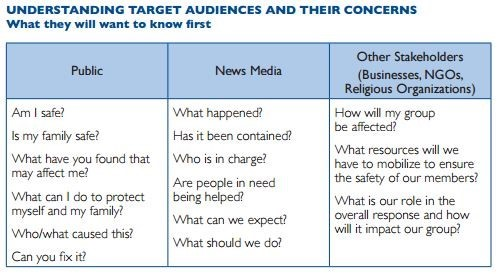
\includegraphics[height=6cm]{informationsNeeds}
\caption{Information needs according to the target audience \cite{panamericanhealthorganization2009}}
\label{fig:informationNeeds}
\end{center}
\end{figure}

The communication of an emergency varies according to the type of incident, the emergency phase and target audience (stakeholders) who will receive the information. The communicator needs
to provide each target audience with relevant information from their perspective, always trying to address their main concerns (Figure \ref{fig:informationNeeds}) in a clear and objective way. Therefore, it is essential to determine which information should be sent to each specific stakeholder, when and using which communication means.

Techniques used for variability modelling in software product line engineering can be useful for modelling commonalities and variabilities in variant-rich scenarios too. Considering the scenario of public communication of emergencies, the benefits of using variability modelling techniques are related to an efficient generation of customised messages for specific audiences, a comprehensive model to consolidate the variation points of the public communication process, and the ability to perform consistency checking of the generated messages.

After gathering the necessary information during the workshop, we decided to model the variability of this domain through feature modelling. This approach is largely used in practice for identifying and describing variability in a set of similar products, and it guided the task of developing a public communication solution capable of addressing the different stakeholders’ needs. 

\subsection*{Configuration Feature Model}

\begin{figure*}[]
\begin{center}
  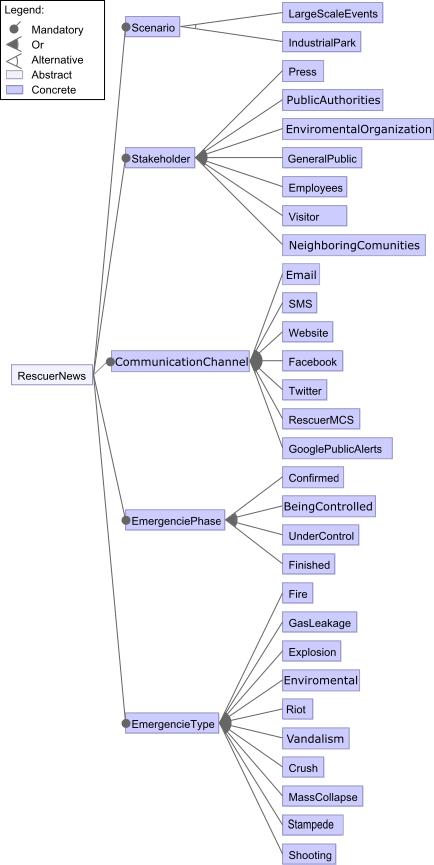
\includegraphics[width=0.7\linewidth]{FMConfiguracao}
\caption{Configuration Feature Model}
\label{fig:FMConf}
\end{center}
\end{figure*}


\begin{table}[]
\centering
\caption{Constraints of the configuration feature model}
\label{constraints}
\begin{tabular}{ll}
\rowcolor[HTML]{9BBB59} 
{\color[HTML]{FFFFFF} Set of Constraints}                                                                                                                 & {\color[HTML]{FFFFFF} Constraints}                                                                                                                                                   \\ \hline
\rowcolor[HTML]{EAF1DD} 
\multicolumn{1}{|l|}{\cellcolor[HTML]{EAF1DD}}                                                                                                            & \multicolumn{1}{l|}{\cellcolor[HTML]{EAF1DD}Large Scale Events EXCLUDES Environmental}                                                                                               \\ \cline{2-2} 
\rowcolor[HTML]{EAF1DD} 
\multicolumn{1}{|l|}{\multirow{-2}{*}{\cellcolor[HTML]{EAF1DD}\textbf{\begin{tabular}[c]{@{}l@{}}Scenario and \\ Emergency Type\end{tabular}}}}           & \multicolumn{1}{l|}{\cellcolor[HTML]{FFFFFF}\begin{tabular}[c]{@{}l@{}}Industrial Park EXCLUDES Crush OR Shooting \\ OR Riot OR Vandalism OR Mass Collapse OR Stampede\end{tabular}} \\ \hline
\rowcolor[HTML]{FFFFFF} 
\multicolumn{1}{|l|}{\cellcolor[HTML]{FFFFFF}\textbf{\begin{tabular}[c]{@{}l@{}}Scenario and \\ Stakeholder\end{tabular}}}                                & \multicolumn{1}{l|}{\cellcolor[HTML]{EAF1DD}Large Scale Events EXCLUDES Environmental Organization}                                                                                  \\ \hline
\multicolumn{1}{|l|}{\cellcolor[HTML]{EAF1DD}}                                                                                                            & \multicolumn{1}{l|}{\begin{tabular}[c]{@{}l@{}}Press or Public Authorities OR \\ Environmental Organizations REQUIRES Email\end{tabular}}                                            \\ \cline{2-2} 
\rowcolor[HTML]{EAF1DD} 
\multicolumn{1}{|l|}{\cellcolor[HTML]{EAF1DD}}                                                                                                            & \multicolumn{1}{l|}{\cellcolor[HTML]{EAF1DD}\begin{tabular}[c]{@{}l@{}}Employees OR Neighbouring Communities \\ REQUIRES Sms OR Rescuer MCS\end{tabular}}                            \\ \cline{2-2} 
\multicolumn{1}{|l|}{\cellcolor[HTML]{EAF1DD}}                                                                                                            & \multicolumn{1}{l|}{\begin{tabular}[c]{@{}l@{}}General Public REQUIRES Website\\ OR Twitter OR Facebook OR \\ Google Public Alerts OR Rescuer MCS\end{tabular}}                      \\ \cline{2-2} 
\rowcolor[HTML]{EAF1DD} 
\multicolumn{1}{|l|}{\multirow{-4}{*}{\cellcolor[HTML]{EAF1DD}\textbf{\begin{tabular}[c]{@{}l@{}}Stakeholder and \\ Communication Channel\end{tabular}}}} & \multicolumn{1}{l|}{\cellcolor[HTML]{EAF1DD}Visitor requires Rescuer MCS}                                                                                                            \\ \hline
\end{tabular}
\end{table}

As aforementioned, emergencies and crises have characteristics in common; however, there are particularities related to the application scenarios and several other aspects. As consequence, we
mapped the variation points to enable the configuration of our solution. Figure \ref{fig:FMConf} presents the resulting model.



Five features (parental features) are essential to define the basic configuration of our solution: scenario, stakeholder (target audience), communication channel, emergency phase and the type of the emergency. The relationship between the Scenario (parent feature) and your child features (or sub-features) is ALTERNATIVE (i.e., only one sub-feature can be selected when configuring for a certain organisation/scenario). Other relationships are OR (i.e., more than one sub-feature can be selected when configuring). The selection of the child features for the 5 parental features defines what will be possible in terms of public communication for the organisation owing the resulting configuration.



Table \ref{constraints} presents the constraints that apply to the configuration feature model. There are emergency types that are directly related to a certain application scenario. In RESCUER, environmental incidents are related to industrial areas, but they are not expected in large-scale events. Based on this observation, we defined two constraints to specify the valid combinations of scenarios (large-scale events and industrial parks) and emergencies types.

Likewise, we specified one constraint between scenario and stakeholders. For example, environmental organisations are not part of the target audience for any communication when the scenario is a large scale event.
The remaining constraints capture valid associations between communication channel and stakeholder. Some communication channels are more efficient to reach particular groups of stakeholders. For example, is highly unlikely that the organisation in charge of a football match in a stadium has the cell phone number or email address of visitors in order to be able to send a SMS or e-mail, but this target audience can be notified by a Mobile Solution based on their geographical position. Based on this observation, we present four constraints to define the set of valid associations.

\subsection*{Variability on the Public Communication Itself}

\begin{figure}[]
\centering
{
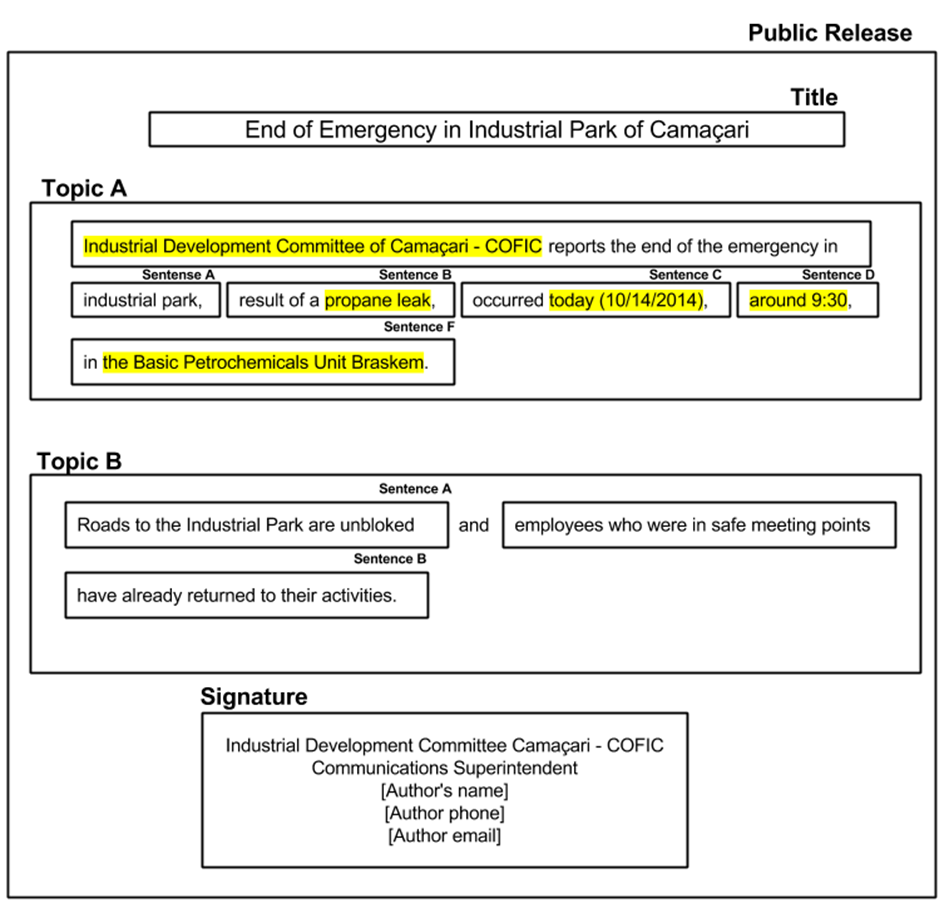
\includegraphics[width=0.5\linewidth]{CoficTemplate}
\label{model1}
}
\caption{Example of COFIC Public Communication Template}
\label{fig:templates}
\end{figure}


We worked on the identification of commonalities and variabilities on the composition of public communication messages. To that end, we analyse a set of templates of our partners (COFIC and FIRESERV) and models proposed in best practice manuals \cite{cisvGuide} \cite{certTemplates} \cite{} in public communication of emergencies in order to identify the structure of this model and the relationships between your information. Figure \ref{fig:templates} present a real example of template used by COFIC in real emergency situations.



After analysing the templates, we defined a generic structure for public communications. This structure consists of the following elements: Title, Topics, Sentences and Signature.

\begin{itemize}
   \item Title: Title of the public communication.
   \item Topic: Set of sentences. Each topic has a communication goal, such as informing the occurrence of an emergency, or the actions taken to control the emergency.
   \item Sentence: Phrase (or part of a phrase) whose content can be changed by the public communicator. 
   \item Signature: Complete signature of the responsible for the public communication.

 \end{itemize}
 

 

 
 First, we observed that the public communication templates change according to the current phase of the emergency. This happens because the goals of communication are different in each emergency phase (Section \ref{cercPhase}). Another important aspect that influences the communication template is the message type. Communications channels such as social networks, SMS, and mobile applications have limitations on the message size or are used in small screens; this implies in short communication templates.
 
  \begin{figure}[]
\centering
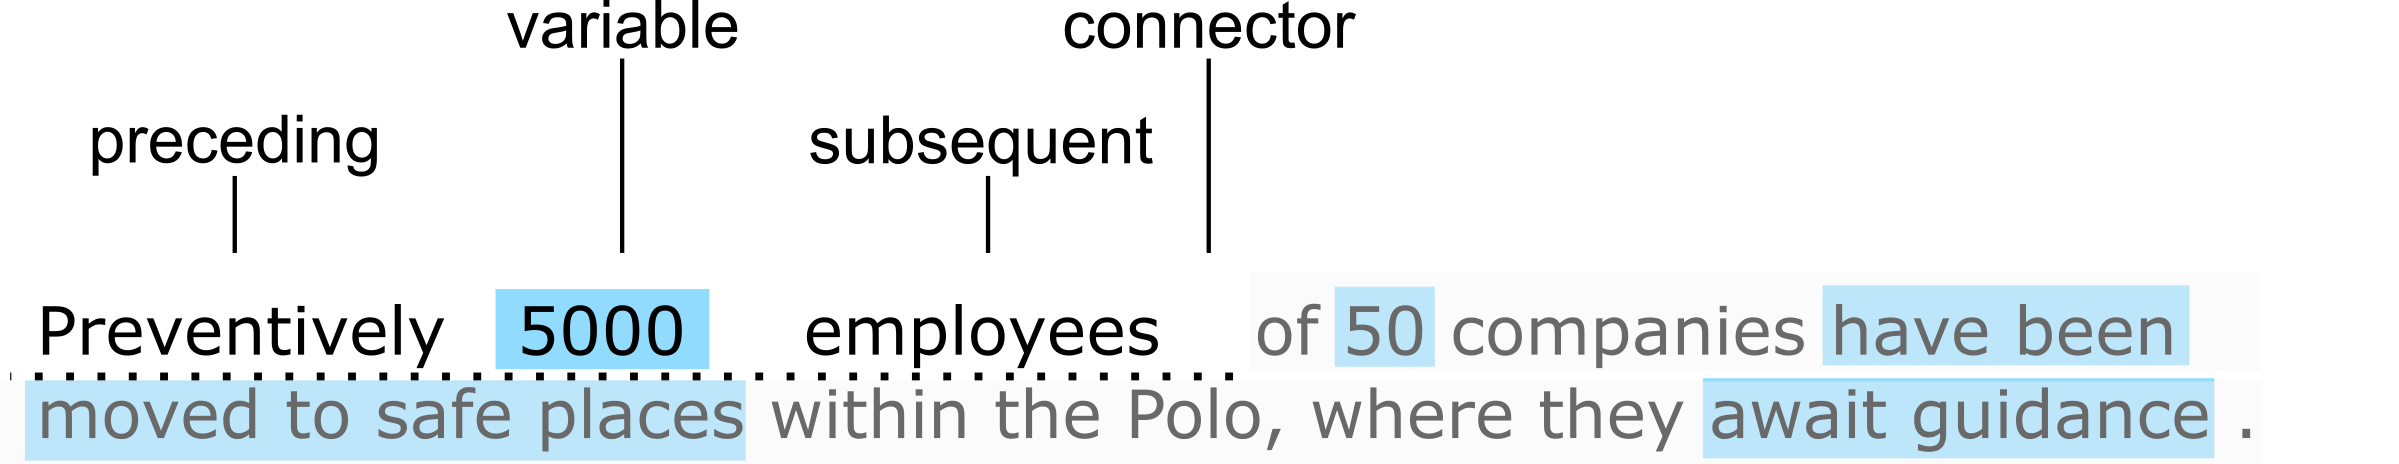
\includegraphics[width=\linewidth]{images/sentenceStructure}
\caption{Setence Structure}
\label{fig:sentencStructure}
\end{figure}

 
 After analysing the public communication templates, we were able to observe that sentences can be structured in: the text preceding the variable information (optional), the variable information (mandatory), the subsequent text (optional) and one connector between sentences (mandatory). Figure \ref{fig:sentencStructure}  shows an example of connected sentences and points out the structure of one of the sentences.
 
 Furthermore, sentences are directly linked to the target audiences, as they have different concerns (Figure \ref{fig:informationNeeds}). Figure \ref{fig:FMModel} presents the result of our variability mapping of the content of public communication messages.
 
    \begin{figure}[]
\begin{center}
  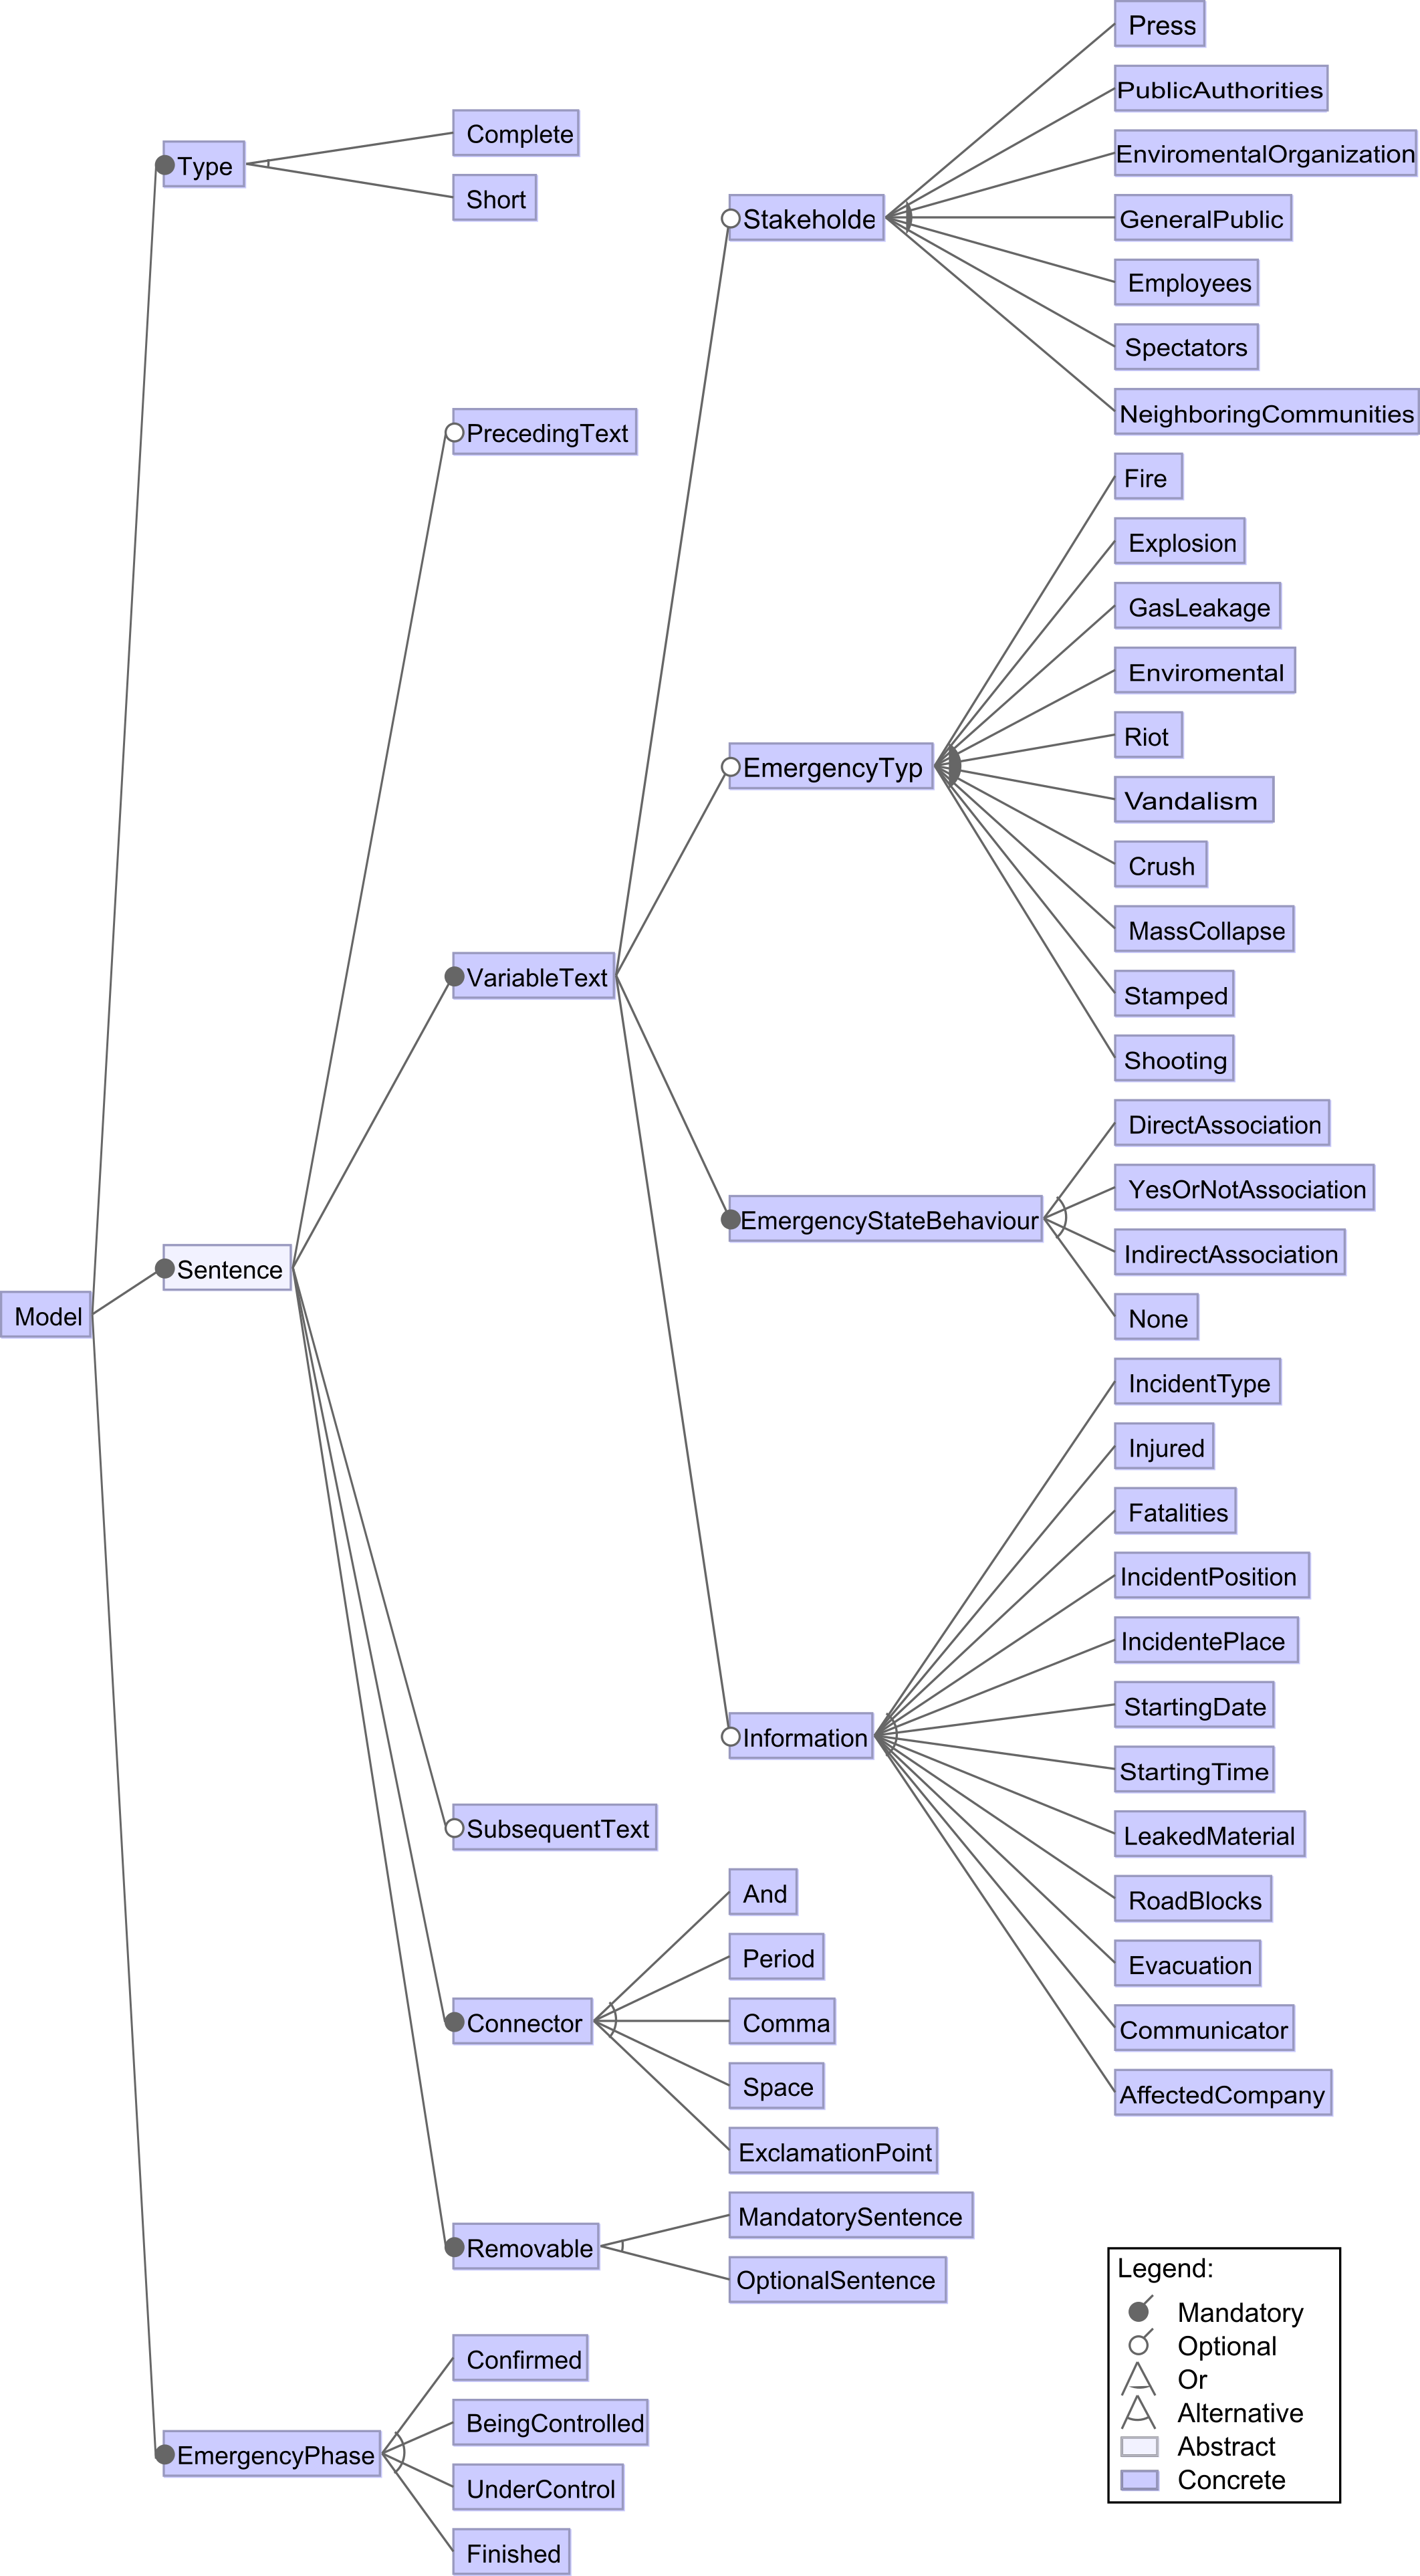
\includegraphics[scale=0.55]{FMModel}
\caption{Content feature model}
\label{fig:FMModel}
\end{center}
\end{figure}
 
\section{Our proposal}

\begin{figure}[]
\begin{center}
  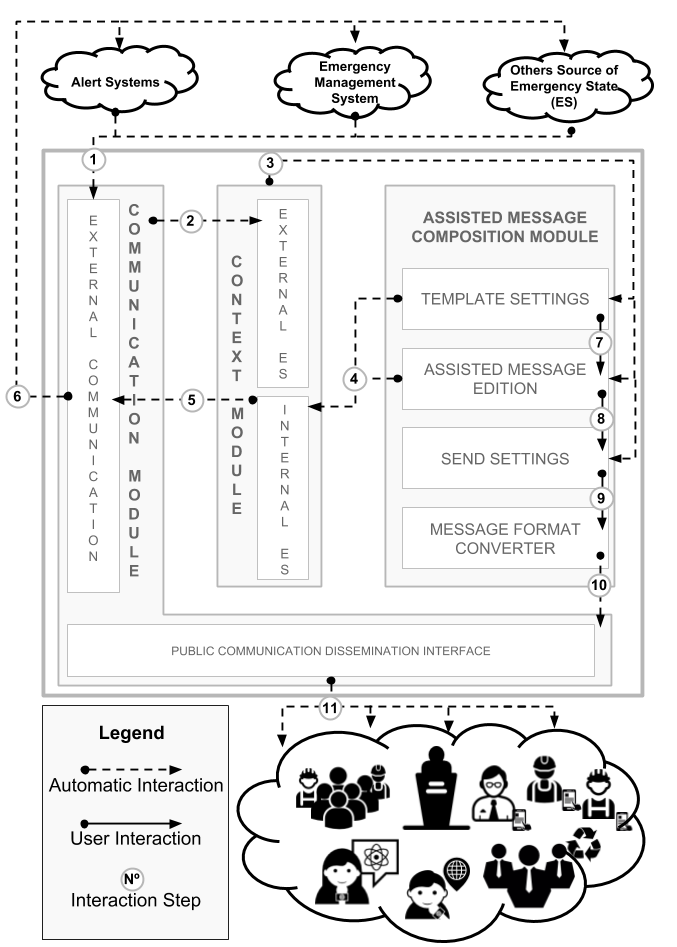
\includegraphics[width=0.9\linewidth, keepaspectratio]{ConceptualModel}
\caption{Proposed Conceptual Model}
\label{fig:ConceptualModel}
\end{center}
\end{figure}

Based on the results of our research of the good practices for public communication of emergencies, in the results obtained in the two workshops carried out with specialists in public communication and our analysis of variability in the whole process of public communication, we propose a computational model that provides a complete support in the task of public communication of emergencies.   

Figure \ref{fig:ConceptualModel} presents our computational model for public communication of crisis and emergencies. We will present our model according to the Steps of Emergencies directly linked to the task of creation and dissemination of public communications: Verify the Situation, Prepare Information and Release Information through Prearranged Channels




\subsection{Verify the Situation}

The task of communicating the public about the occurrence of an emergency and its consequences begins with the search of reliable information. Situational awareness is essential to guarantee that only consistent information will be transmitted to the public and thereby achieve gain the public's confidence. 

In some cases, the reliable information can be obtained in other software of emergency management or alert systems. Because of this, the first interaction described in our model is an automatic search of information in external systems. The responsibility of the communication module, more specifically, the sub-module of External Communication is to implemented interfaces that periodically and automatically get information from external sources and provide it to the context module (interaction 2). 

The set of information obtained from external source compose the External Knowledge in the Context Module. We call from Internal Knowledge the information obtained by the input of the users during the interaction within the Assisted Message Composition Module (AMC) (Interaction 5). The Context Module is responsible for automatically management the information of the Internal and External Knowledge and to provide the most recent information to the AMC module (Interaction 3).

Commonly, some information about the emergency is not obtained from External Source of information. This information probably will be put during the composition of emergency public communication by the emergency communication team. In this case, is important share this information for the others Emergency Management Systems. Because of this, the Internal Knowledge is automatically sent to the External Communication Sub-module (interaction 6) which, in sequence, share this information with external systems (interaction 7).



\subsection{Prepare Information}

The main contribution of our work is the semi-automated approach to building public communications. We map the variability in the composition of public communications messages and as result, we create structured templates that adapt to the current emergency state in order to reduce the necessity of interactions to compose the public communication.

The process of creation of public communications begins with the configuration of the Template Message. As noted above in the mapping of variability, some characteristics are essential to define the appropriate template for the current emergency. We generate the most appropriated model according to the response of 4 questions: What happened? ( what is the type of emergency); What is the current status? (what is the current phase of emergency); and which and how the target audience will be communicated. Some of this questions are linked to the emergency state and then the Template Settings sub-module can consume (interaction 3) or provide (interaction 5) information to the Context Module. 

After obtaining the essential information about the communication of emergency, the Assisted Message Edition sub-module generate a dynamic template according to these information (interaction 4). This process includes the exclusion of sentences exclusive for specifics target audiences (that are not targets of this communication) or emergency type (different of present emergency).

In addition, it is necessary to configure the sentences according to the present emergency status. We observed a relationship between emergency characteristics and the content of public communications in the variability of content according to the status of emergency. There are four generic types of variation in the content of a sentence depending on the state of the emergency, the variation can be either: 

\begin{enumerate}
   \item A direct association, where the value of the variable information is an emergency state data;
   \item An indirect association, in which the value of the variable information depends on an emergency state data, but it have not the same value;
   \item Based on the occurrence (or not) of a fact, which might come from the emergency state;
   \item An information not associated with the emergency state.
\end{enumerate}

Figure \ref{fig:sentenceContext} shows practical examples of each different behaviour identified and its influence on the content of the sentences.

\begin{figure}[]
\centering
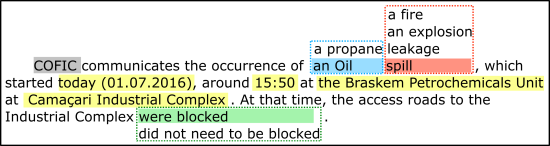
\includegraphics[width=\linewidth]{images/sentences}
\caption{Examples of different behaviour on the content of sentences according to the emergency status}
\label{fig:sentenceContext}
\end{figure}

The information marked in yellow in the example are the content that has a direct association with the emergency state, like emergency start date and time, the name of the affected company and so on. This information was put directly into the content of the sentence.

In red, we present an example of indirect association between emergency state and part of the sentence. The sentence will read "a fire" in case the emergency type is "FIRE", "an explosion" in case the emergency type is EXPLOSION", "leakage" in case of "GAS LEAKAGE" emergency, and "spill" in case the emergency type is "ENVIRONMENTAL”. 

An example of a sentence that the variable content is based on the occurrence or not of a fact is given in green. In this case, the occurrence or not of road blocks. 

An example of sentence not associated with the emergency state is given in grey. The name of the company that is responsible for handling the crisis, in this case, is an information about the system configuration (e.g. the company that the RESCUER News user is associated).

Finally, an example of qualifier for the emergency type is showed in blue. The leaked material is a type of information associated with the incident "GAS LEAKAGE" or "ENVIRONMENTAL".



\subsection{Release Information through Prearranged Channels}

Disseminate the public communication through the most appropriate communication channel for each target audience is essential to help ensure the successful in the public communication of an emergency.

In the Send Setting sub-module, the user can select the dissemination area, email and cell-phone list and other configurations of the selected communication channels. After that (interaction 9) the Message Format Converter (MFC) sub-module generate the specific message for each target audience from the Structured Template ( a result of the Assisted Message Edition sub-module).  After that, the MFC needs to convert each message to the appropriated format to be send by each communication channel (interaction 10). 

Finally, the messages are sent automatically by the Public Communication Dissemination Interface (interaction 11). Is in this Interface that is implemented the logic to send messages for each communication channel. 







\section{Conclusion and Activity Schedule}

Public communication is a key activity in emergency and crisis management. The challenge of this activity is to establish a good strategy for communication with the partners that should be informed. A crucial aspect is to ensure that the right people will receive the information they need, when they need it.

We specified in detail the variabilities that support the configuration to different scenarios and organisations, as well as the variabilities that allow the sending of customised public communications in a semi-automatic way, taking into account emergency state, target audience and communication channel.

When compared with the existing solutions for public communication, our proposed brings the benefit of using dynamics templates to allow the semi-automatic and flexible creation of public communications taking into consideration the target audience, incident type, emergency phase and adapt the content of the message according to emergency state information.

The Figure \ref{fig:Schendule} presents our activity diagram to the remainder of the masters course.

\begin{figure}[!h]
\begin{center}
  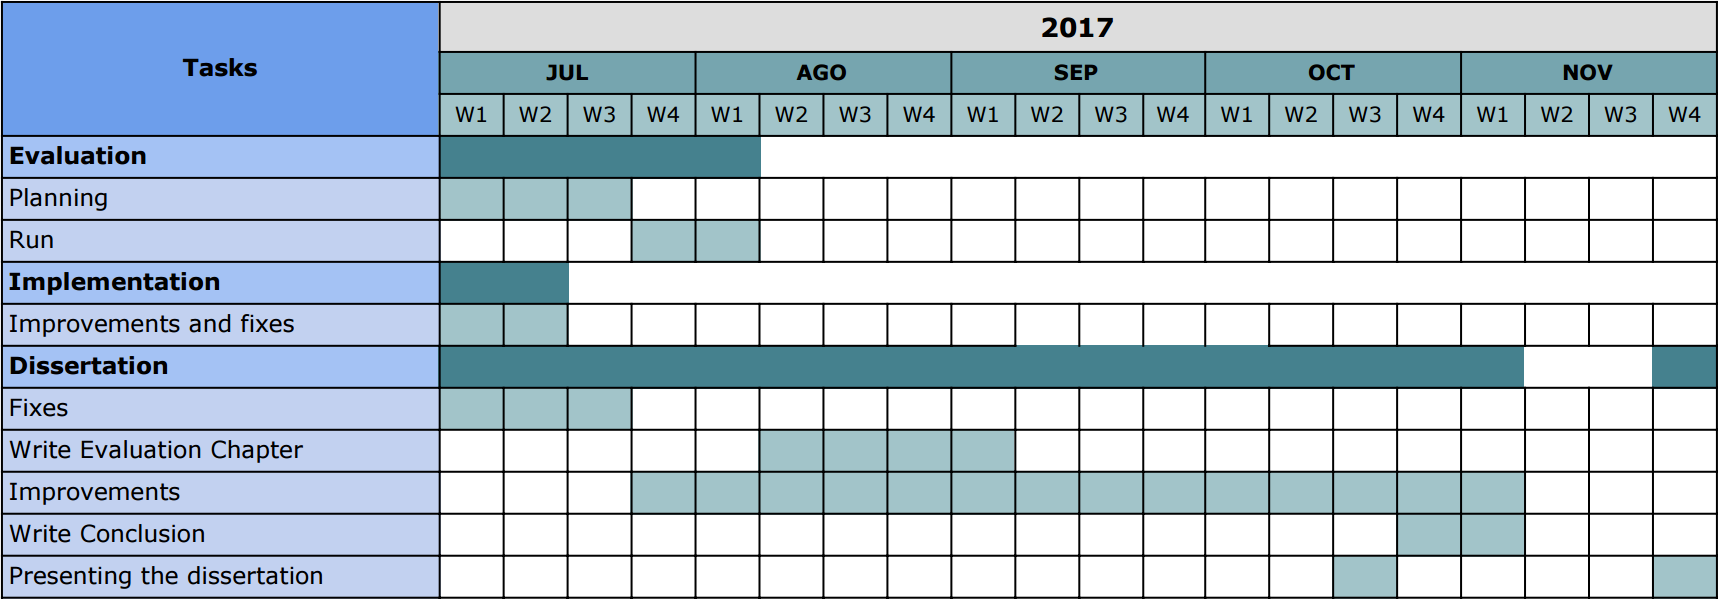
\includegraphics[width=\linewidth, keepaspectratio]{Cronograma}
\caption{Activity Schedule}
\label{fig:Schendule}
\end{center}
\end{figure}


The next step of our research is improving our implementation according to the feedback of specialist, collected during demonstrations of the Rescue Project. In parallel, we will plan the evaluation of our research. We will run the evaluation with specialists of emergency in Industrial Parks and Large Scale Events( the scenarios that this research was developed) and specialists from Civilian Defence (new scenario). The last evaluation, in a new scenario, is intended to verify if our proposal is valid in others types of emergency. Finally, the last step of our research is writing the results of the evaluation and conclude the writing of our master thesis. 

